\paragraph{Checkpoint follow-up.}
Eight seed groups had higher selected test loss with exchange. Two kept the same selected index, with gaps \(+0.01162\) and \(+0.00037\). For the six that changed index, I also scored the exchange checkpoint at the independent arm's chosen index on the same 32 test minibatches, using 192 additional test forwards and zero gradient evaluations.

Let \(i\) and \(j\) be the validation-selected indices in the exchange (\(S\)) and independent (\(I\)) runs. With \(L\) denoting test loss, Figure~\ref{fig:checkpoint-gaps} shows the two terms below and their sum.
\[
 L_S(i)-L_I(j)
 =\underbrace{L_S(j)-L_I(j)}_{\text{fixed-index gap}}
 +\underbrace{L_S(i)-L_S(j)}_{\text{reselection gap}}.
\]

\begingroup
\setlength{\intextsep}{5pt}
\begin{figure}[!ht]
\centering
\setlength{\abovecaptionskip}{3pt}
\small
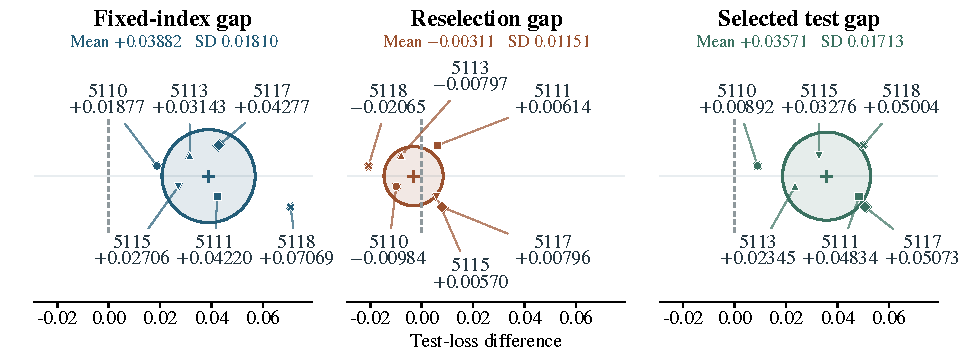
\includegraphics[width=0.96\linewidth]{nanogpt_checkpoint_gaps.pdf}
\caption{Test-loss gaps for six groups with higher selected loss and a changed index. Crosses mark means, and circle radii are one sample SD. Labels give the seed and its signed horizontal coordinate. Vertical offsets separate points. Sample variances from left to right are \(3.28\), \(1.32\), and \(2.93\) in units of \(10^{-4}\).}
\label{fig:checkpoint-gaps}
\end{figure}
\endgroup

The fixed-index test loss rose in all six groups. Reselection reduced test loss in three and increased it in three, offsetting \(0.00311\) on average. The local gradient alignment remains unmeasured.
